	\chapter{Kravspecifikation}
	
	\section{Systembeskrivelse}
	Systemet består af en database med brugeradgang via en iOS applikation.
	Databasen indeholder brugere, sager og data om de forskellige projekt registreringer.
	En registrering kan indeholde; tekst, billeder, GPS lokation og mulighed for at give det en status.
	
	\subsection{Domain model}
	Herunder ses et rigt billede af systemet som skal udvikles.
	\begin{figure}[h!]
		\centering
		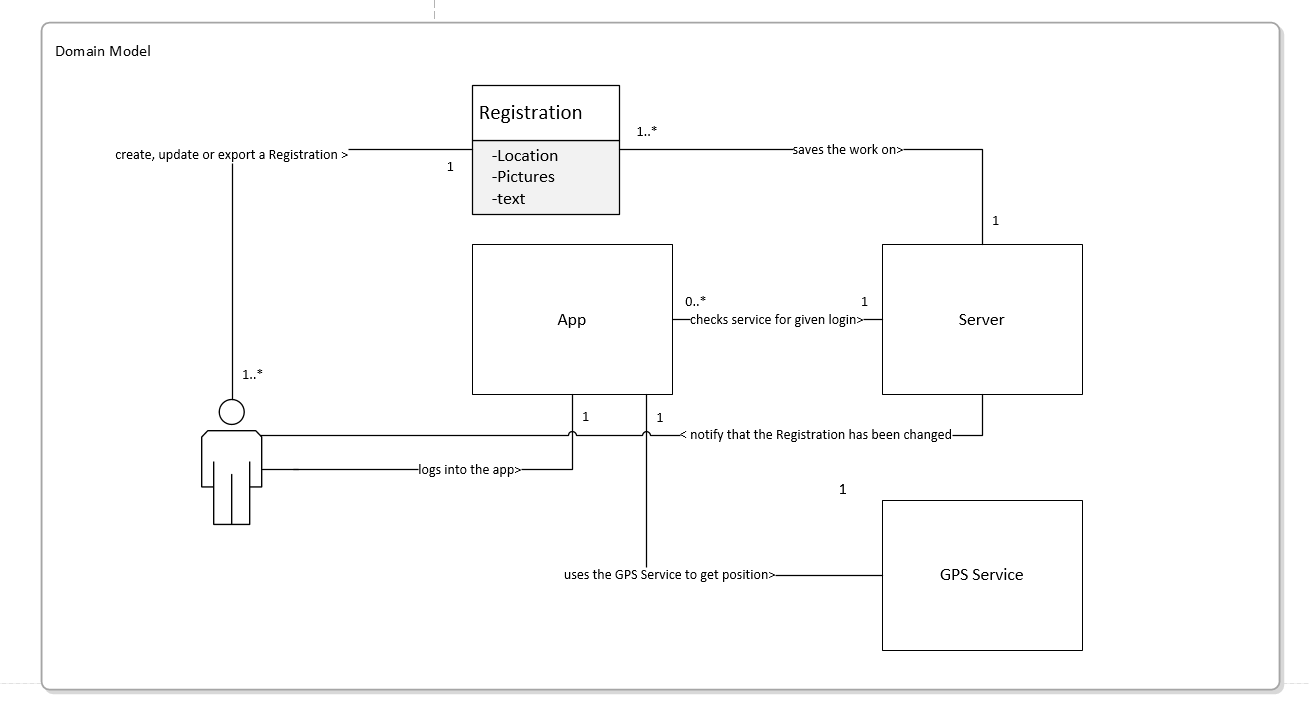
\includegraphics[width=1\linewidth]{Kravspecifikation/Domainmodel}
	\end{figure}	
	
	\section{User stories} 
	Følgende er en beskrivelse kort af user stories til Rambøll's applikation:

	\subsection*{Log-in (CRS-1)}
	Som bruger\\
	Ønsker jeg at kunne logge ind på applikationen\\
	For at kunne benytte applikationen
	
	\subsection*{Opret registrering (CRS-2)}
	Som ejer\\
	Ønsker jeg at kunne oprette en registrering\\
	For at kunne skrive en kommentar til et byggeprojekt
	
	\subsection*{Opdatere registrering (CRS-3)}
	Som ejer\\
	Ønsker jeg at kunne opdatere en registrering\\
	For at kunne ændringer de oplysninger der er på en given registrering
	
	\subsection*{Eksportere registrering (CRS-4)}
	Som ejer\\
	Ønsker jeg at kunne ekspotere en registrering\\
	For at kunne dele registreringen med andre parter af projektet
	
	\subsection*{Modtage opdateringer (CRS-5)}
	Som bruger\\
	Ønsker jeg at kunne modtage opdateringer\\
	For at kunne være opdateret omkring en registreringen
	
	\subsection*{GPS Lokation (CRS-6)}
	Som bruger\\
	Ønsker jeg at kunne se min positionen \\
	For at kunne sætte en præcis lokation på en registreringen. \\
	
	\section{Ikke-funktionelle krav}
	\begin{itemize}[-]
		\itemsep 0.3em 
		\item Skal kunne tilgås gennem en iOS applikation \textbf{(TRS-1)}
		\item Der vil blive anvendt Microsoft Visual Studio med et Xarmarin plugin til udvikling af applikationen. \textbf{(TRS-2)}
		%\item Der vil blive anvendt Microsoft SQL udvikling af databasen. \textbf{(TRS-3)}
		\item Alle brugere skal kunne anvende systemet på samme tid. Maks antal enheder er 20 på samme tid \textbf{(TRS-4)}
	\end{itemize}
	